\documentclass[10pt,twocolumn,letterpaper]{article}

\usepackage{cvpr}
\usepackage{times}
\usepackage{epsfig}
\usepackage{graphicx}
\usepackage{amsmath}
\usepackage{amssymb}
\usepackage{listings}

% Include other packages here, before hyperref.

% If you comment hyperref and then uncomment it, you should delete
% egpaper.aux before re-running latex.  (Or just hit 'q' on the first latex
% run, let it finish, and you should be clear).
\usepackage[breaklinks=true,bookmarks=false]{hyperref}

\cvprfinalcopy % *** Uncomment this line for the final submission

\def\cvprPaperID{****} % *** Enter the CVPR Paper ID here
\def\httilde{\mbox{\tt\raisebox{-.5ex}{\symbol{126}}}}

% Pages are numbered in submission mode, and unnumbered in camera-ready
%\ifcvprfinal\pagestyle{empty}\fi
\setcounter{page}{1}
\begin{document}

%%%%%%%%% TITLE
\title{
Identify Obstacles And Grab Items By Robot Arms \\
\bigskip
\large A project of the	2017 Robotics Course of	the	School of \\
Information Science and Technology (SIST) \\
of ShanghaiTech University}


\author{Haihao Zhu\\
{\tt\small zhuhh2@shanghaitech.edu.cn}
% For a paper whose authors are all at the same institution,
% omit the following lines up until the closing ``}''.
% Additional authors and addresses can be added with ``\and'',
% just like the second author.
% To save space, use either the email address or home page, not both
\and
Hudie Gu\\
{\tt\small guhd@shanghaitech.edu.cn}
\and
Yi Yang\\
{\tt\small yangyi1@shanghaitech.edu.cn}
}
\maketitle
%\thispagestyle{empty}

%%%%%%%%% ABSTRACT
\begin{abstract}
   This project is based on Dobot Magician Robot Arm and Ros, we plan to create a model by usig URDF file in Ros invironment, and make the model move along the real robot.
   
\end{abstract}

%%%%%%%%% BODY TEXT
\section{Introduction}

\subsection{Dobot}
The Dobot Magician Robot Arm is multi-task robot arm that has black and white body with consistent qualityat fingertipsUnibody design, unbox and enjoy right away Designed for desktop, safe and easily lifted. It contains a Vacuum pump Kit , Gripper, Wirting and Drawing Kit, 3D Printing Kit, and other accessories.

It has many features like writing, drawing, 3D printing and even playing chessing with human.  


\subsection{URDF}

URDF means Unified Robot Description Format, it is Kinematic and basic physics description of a robot in XML file format. It mainly consists of tags like links , joint and material.  Many of the coolest and most useful capabilities of ROS and its community involve things like collision checking and dynamic path planning. It’s frequently useful to have a code-independent, human-readable way to describe the geometry of robots and their cells. Think of it like a textual CAD description: “part-one is 1 meter left of part-two and has the following triangle-mesh for display purposes.” The Unified Robot Description Format (URDF) is the most popular of these formats today. This module will walk you through creating a simple robot cell that we’ll expand upon and use for practical purposes later.

\section{State of the art}

Since the initial goal of this project is trying to identify obstacles and grasp items by robot arms, but situation changes when the initial robot arm is broken. Then we changed our goal to model the new Dobot robot arm and make it move along the real Maigician Dobot Arm, which has no State-Of-The-Art part, so we list the content in the intermidiate report.

\subsection{Haihao Zhu}

\begin{enumerate}
\item \textbf{Motion Planning of Humanoid Robot Arm for grasping task} \cite{4516345}

This paper demonstrates a new method for computing numerical solution to the motion planning of humanoid robot arm. The method is based on combination of two nonlinear programming techniques which are Forward recursion formula and FBS method. 

\item \textbf{Autonomous vision-guided bi-manual grasping and manipulation} \cite{8025192}

This paper describes the implementation, demonstration and evaluation of a variety of autonomous, vision-guided manipulation capabilities, using a dual-arm Baxter robot. It starts from the case that human operator  moves the master arm and slave arm follows the master arm, and then, it combines an image-based visual servoing scheme with the first case to perform dual-arm manipulation without human intervention. 
  
\item \textbf{Arm grasping for mobile robot transportation using Kinect sensor and kinematic analysis} \cite{7151321}

In this paper, we describe how the grasping and placing strategies for 6 DOF arms of a H20 mobile robot can be supported to achieve a high precision performance for a safe transportation. An accurate kinematic model has bean used in this paper to find safe path from one pose to another precisely.

\item \textbf{A new method for mobile robot arm blind grasping using ultrasonic sensors and Artificial Neural Networks} \cite{6739654}

The paper presents a new method to realize mobile robot arm grasping in indoor laboratory environments. This
method adopts a blind strategy, which does not need the robot arms be mounted any kind sensors and avoid calculating the complex kinematic equations of the arms.

The method includes:
\begin{enumerate}
\item two robot on-board ultrasonic sensors in base are utilized to measure the distances between the robot base and the front arm grasping tables; 

\item an Artificial Neural Networks (ANN) is proposed to learn/establish the nonlinear relationship between
the ultrasonic distances and the joint controlling values. After executing the training step using sampling data, the ANN can forecast/generate the next-step joint controlling values fast and
accurately by inputting a new pair of real-time ultrasonic measured distances; 

\item to let the blind strategy matching with the transportation process, an arm controlling component with
user interfaces is developed;

\item a method named training arm is adopted to prepare the training data for the training procedure of the ANN model.

Finally, an experiment proves that the proposed strategy has good performance in both of the accuracy and the real-time computation, which can be applied to the real-time arm operations for the mobile robot transportation in laboratory automation.

\end{enumerate}

\item \textbf{find-object}
 
Find-object is a Simple Qt interface to try OpenCV implementations of SIFT, SURF, FAST, BRIEF and other feature detectors and descriptors.

it have many features like:

\begin{enumerate}
\item You can change any parameters at runtime, make it easier to test feature detectors and descriptors without always recompiling.

\item Detectors/descriptors supported (from OpenCV): BRIEF, Dense, FAST, GoodFeaturesToTrack, MSER, ORB, SIFT, STAR, SURF, FREAK and BRISK.

\item Sample code with the OpenCV C++ interface below...

\item For an example of an application using SURF descriptors: see my project RTAB-Map (an appearance-based loop closure detector for SLAM).
\end{enumerate}

\end{enumerate}

\subsection{Yi Yang}

\begin{enumerate}
\item Dynamic Sensor-Based Control of Robots with Visual Feedback

This paper describe the formulation of sensory feedback models for systems which incorporate complex mappings between robot, sensor, and world coordinate frames. These models explicitly address the use of sensory features to define hierarchical control structures, and the definition of control strategies which achieve consistent dynamic performance. Specific simulation studies examine how adaptive control may be used to control a robot based on image feature reference and feedback signals. 

\item Vision-based Motion Planning For A Robot Arm Using Topology Representing Networks

This paper describe the concept of the Perceptual Control Manifold and the Topology Representing Network. By exploiting the topology preserving features of the neural network, path planning strategies defined on the TRN lead to flexible obstacle avoidance. The practical feasibility of the approach is demonstrated by the results of simulation with a PUMA robot and experiments with a Mitsubishi Robot. 

\item A Framework for Robot Motion Planning with Sensor Constraints

This paper propose a motion planning framework that achieves this with the help of a space called the perceptual control manifold (PCM) defined on the product of the robot configuration space and an image-based feature space. They show how the task of intercepting a moving target can be mapped to the PCM, using image feature trajectories of the robot end-effector and the moving target. This leads to the generation of motion plans that satisfy various constraints and optimality criteria derived from the robot kinematics, the control system, and the sensing mechanism, specific interception tasks are analyzed to illustrate this vision-based planning technique. 

\item Motion Planning of a Pneumatic Robot Using a Neural Network

This paper present a framework for sensor-based robot motion planning that uses learning to handle arbitrarily configured sensors and robots. Autonomous robotics requires the generation of motion plans for achieving goals while satisfying environmental constraints. Classical motion planning is defined on a configuration space which is generally assumed to be known, implying the complete knowledge of both the robot kinematics as well as knowledge of the obstacles in the configuration space. Uncertainty, however, is prevalent, which makes such motion planning tech­niques inadequate for practical purposes. Sensors such as cameras can help in over­coming uncertainties but require proper utilization of sensor feedback for this purpose. A robot motion plan should incorporate constraints from the sen­sor system as well as criteria for optimizing the sensor feedback. However, in most motion planning approaches, sensing is decoupled from planning. A framework for motion planning was proposed that considers sensors as an integral part of the: definition of the motion goal. The approach is based on the concept of a Perceptual Control Manifold (PCM), defined on the product of the robot configuration space and sensor space. The PCM provides a flexible way of developing motion plans that exploit sensors effectively. However, there are robotic systems, where the PCM cannot be derived analytically, since the exact mathematical relation­ship between configuration space, sensor space, and control signals is not known. Even if the PCM is known analytically, motion planning may require the tedious and error prone process of calibration of both the kinematic and imaging parameters of the system. Instead of using the analytical expressions for deriving the PCM, they therefore propose the use of a self-organizing neural network to learn the topology of this manifold. They first develop the general PCM concept, then describe the Topology Representing Network (TRN) algorithm they use to approximate the PCM and a diffusion-based path planning strategy which can be employed in conjunction with the TRN. Path control and flexible obstacle avoidance demonstrate the feasibility of this approach for motion planning in a realistic environment and il­lustrate the potential for further robotic applications.

\item $ usb\_cam $

The “usb\underline{\hspace{0.5em}}cam” package, usually together used with “cv\underline{\hspace{0.5em}}camera” package, is a driver used to make the camera capture the real environment and use the data transmitted by the camera to form a picture. It will create a “usb\underline{\hspace{0.5em}}cam\underline{\hspace{0.5em}}node”. The “usb\underline{\hspace{0.5em}}cam\underline{\hspace{0.5em}}node” interfaces with standard USB cameras using “libusb\underline{\hspace{0.5em}}cam” and publishes images as “sensor\underline{\hspace{0.5em}}msgs::Image”. Uses the “image\underline{\hspace{0.5em}}transport” library to allow compressed image transport. The published topics is “<camera\underline{\hspace{0.5em}}name>/image”. It has lots of parameters, “video\underline{\hspace{0.5em}}device (string, default: "/dev/video0")” to choose the device the camera is on; “image\underline{\hspace{0.5em}}width (integer, default: 640)” and “image\underline{\hspace{0.5em}}height (integer, default: 480)” to set image width and image height; “pixel\underline{\hspace{0.5em}}format (string, default: "mjpeg")” to change the picture format which possible values are mjpeg, yuyv, uyvy; “io\underline{\hspace{0.5em}}method (string, default: "mmap")” to change the input and output method which possible values are mmap, read, userptr; “camera\underline{\hspace{0.5em}}frame\underline{\hspace{0.5em}}id (string, default: "head\underline{\hspace{0.5em}}camera")” to set the camera's tf frame; “framerate (integer, default: 30)” to change the required framerate; “contrast (integer, default: 32)” to set the contrast of video image (0-255); “brightness (integer, default: 32)” to set brightness of video image (0-255); “saturation (integer, default: 32)” to set saturation of video image (0-255); “sharpness (integer, default: 22)” to set sharpness of video image (0-255); “autofocus (boolean, default: false)” to determine whether enable camera's autofocus or not; “focus (integer, default: 51)” to set the focus of the camera (0=at infinity) if autofocus is disabled. “camera\underline{\hspace{0.5em}}info\underline{\hspace{0.5em}}url (string, default: )” is an url to the camera calibration file that will be read by the CameraInfoManager class; “camera\underline{\hspace{0.5em}}name (string, default: head\underline{\hspace{0.5em}}camera)” is the camera name and must match the name in the camera calibration. The related packages “cv\underline{\hspace{0.5em}}camera” is used to supports image capture from usb cameras using OpenCV. To use the package, first “git clone https://github.com/bosch-ros-pkg/usb\underline{\hspace{0.5em}}cam.git usb\underline{\hspace{0.5em}}cam” to clone the “usb\underline{\hspace{0.5em}}cam” package. Then  build the package. Afterwards, build .launch file. An example is like behind:

\lstset{
    xleftmargin=2em,xrightmargin=2em, aboveskip=1em,
    framexleftmargin=2em
} 

\begin{lstlisting}
$<launch>
$  <node name="usb_cam" pkg="usb_cam" 
        type="usb_cam_node" output="screen" >
$    <param name="video_device" value="/dev/video0" />
$    <param name="image_width" value="640" />
$    <param name="image_height" value="480" />
$    <param name="pixel_format" value="mjpeg" />
$    <param name="camera_frame_id" value="usb_cam" />
$    <param name="io_method" value="mmap"/>
$  </node>
$  <node name="image_view" pkg="image_view" type="image_view"
        respawn="false" output="screen">
$    <remap from="image" to="/usb_cam/image_raw"/>
$    <param name="autosize" value="true" />
$  </node>
$</launch>
\end{lstlisting}

\begin{flushleft}
Finally, use “roslaunch usb\underline{\hspace{0.5em}}cam.launch” to launch.
\end{flushleft}

\end{enumerate}

\subsection{Hudie Gu}

\begin{enumerate}
\item Vision\- based adaptive grasping of a humanoid robot arm

This paper presents a motion planning and control design of a humanoid robot arm for vision-based grasping in an obstructed environment. This study proposes a design for safe operation of the robot arm in an unknown environment, and practical experiments show that the six degree- of-freedom robot arm can effectively avoid obstacles and complete the grasping task.

\item The intelligent robot arm based on sense of sight

This paper designed This paper designs an intelligent robot arm system based on visual sensor,  which can achieve the object's searching and positioning through vision system. In the scheme design, a camera is install above the work area of robot arm, which captures the image of work area in real time. Image segmentation and feature extraction is done by MATLAB to recognize objects. 

\item Optimal trajectory generation for energy consumption minimization and moving obstacle avoidance of a 4DOF robot arm

In this paper, trajectory generation for a 4 DOF arm of SURENA III humanoid robot with the purpose of optimizing energy and avoiding a moving obstacle is presented. This paper use Lagrange approach to model dynamic behavior of a robotic manipulator and a Genetic Algorithm to optimize robot's movements.

\item Multi objective optimization of humanoid robot arm motion for obstacle avoidance

This paper proposed the neural controllers for mobile humanoid robot arm in presence of obstacle and optimizing time, distance and acceleration simultaneously.

The optimization problem is the arm motion generation for obstacle avoidance. To solve it, this research utilized a feedforward neural network(FFNN)while using Laser Range Finder to determine the position of the target. Both hands generate a set of optimized FFNN while each FFNN receives three input.

To solve obstacle avoidance, this research divided the obstacle area in lateral plan in 6 parts and a single pre-evolved neural controller is generated for each section. Then the robot determines the partitions that the obstacle covers based on the obstacle position and size. The robot arm motion is generated based on the specific neural controller reaching the goal position while avoiding the obstacle. 

\item Moveit!

MoveIt! is state of the art software for mobile manipulation, incorporating the latest advances in motion planning, manipulation, 3D perception, kinematics, control and navigation. \par
Primary users can use this interface both through C++ and Python through the move\_ group\_ interface.\par
MoveIt! comes with a plugin for the ROS Visualizer (RViz). The plugin allows users to setup scenes in which the robot will work, generate plans, visualize the output and interact directly with a visualized robot. In this plugin, there are four  different visualizations active:\par
1.The start state for motion planning;\par
2.The goal state for motion planning;\par
3.The robot’s configuration in the planning scene/ planning environment;\par
4.The planned path for the robot.\par
\end{enumerate}

\section{System	Description}

In this project, We intend to realize the following three goals. First of all, we plan to control the robot-arm by human with keyboard manually. Afterwards, we want the robot-arm to automatically seek and fetch the object in the same plane. Besides, we hope the robot-arm can achieve the function that moving the object to a specific location while recognizing and avoiding obstacles.

We will use Ros, moveit, and maybe find-object to achieve the goal above. We will use Ros to control the whole robot arm, and use Moveit package to do motion planning, manipulation, and even collision detection. If we have time, we will try to use find-object package to find multiple object.

For motion planning, we will probably use OMPL(Open Motion Planning Library) algorithm which is the default of Moveit!. For Collision Checking, we will use FCL(Flexible Collision Library) of Moveit! to find check whether there exists collision in planning pat based on the OctoMap generated by 3D Perception plugin.

For computer vision task,  we will use apriltags to find where the tube are relavant to camera.


\section{System	Evaluation}

\subsection{URDF model}

We have built a URDF model by creating URDF file with real size, To simplify, we use cylinder and box to represent links of the arm. It looks like below:

\begin{figure}[t]
\begin{center}
	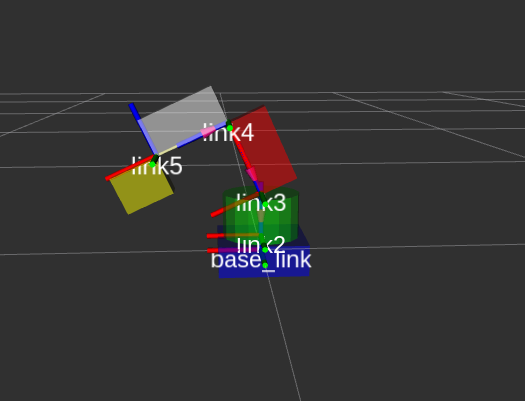
\includegraphics[width=0.8\linewidth]{urdf_model.png}
\end{center}
   \caption{URDF model of the Dobot Magician Arm}
\label{fig:long}
\label{fig:onecol}
\end{figure}

We can see from the figure 1, dobot magician robot arm has a fice links including base link and 4 joint between each of them. To achieve our goal, we need to get the joint message of each joint of the real robot and set it into the joint of URDF model by using $ joint_state_publisher $ package in URDF file.

\subsection{Dobot API}

The main point is how to get joint message of the real robot. We can get it by Dobot API. Since it is ugly to put the code here, I have put the code we write in my git repository \cite{}.

\section{Conclusion}

Finaly, we have achieved our goal that the mode move along the real robot when we press keyboard to control the real robot. The demo can be found in our webpage of this project \cite{}


{
\bibliographystyle{ieee}
\bibliography{final}
}
\end{document}
